\documentclass[10pt, aspectratio=169, handout]{beamer}
\usefonttheme{professionalfonts}
%\usetheme{CambridgeUS}
%
% Choose how your presentation looks.
%
% For more themes, color themes and font themes, see:
% http://deic.uab.es/~iblanes/beamer_gallery/index_by_theme.html
%
\mode<presentation>
{
  \usetheme{Berkeley}      % or try Darmstadt, Madrid, Warsaw, ...
  \usecolortheme{beaver} % or try albatross, beaver, crane, ...
  \usefonttheme{default}  % or try serif, structurebold, ...
  \setbeamertemplate{navigation symbols}{}
  \setbeamertemplate{caption}[numbered]
} 

\setbeamertemplate{footline}{%
  \leavevmode%
  \hbox{%
    \begin{beamercolorbox}[wd=.85\paperwidth,ht=2.5ex,dp=1ex,left]{author in head/foot}%
      \usebeamerfont{author in head/foot}Maxx Seminario, Electronic Circuits, Fall 2025%
    \end{beamercolorbox}%
    \begin{beamercolorbox}[wd=.15\paperwidth,ht=2.5ex,dp=1ex,right]{date in head/foot}%
      \hspace*{0.5em}\insertframenumber{} / \inserttotalframenumber\hspace*{0.5em}%
    \end{beamercolorbox}%
  }%
  \vskip0pt%
}

\usepackage[english]{babel}
\usepackage[utf8x]{inputenc}
\usepackage{tikz}
\usepackage{pgfplots}
\usepackage{array}  % for table column M
\usepackage{makecell} % to break line within a cell
\usepackage{verbatim}
\usepackage{graphicx}
\usepackage{subcaption}
\usepackage{amsfonts}
\usepackage{amsmath}
\usepackage{bm}
\usepackage{epstopdf}
\usepackage{circuitikz}
\usepackage{caption}
\captionsetup{compatibility=false}
%\usepackage{dsfont}
\usepackage[absolute,overlay]{textpos}
\usetikzlibrary{calc}
\usetikzlibrary{pgfplots.fillbetween, backgrounds}
\usetikzlibrary{positioning,arrows.meta}

\usetikzlibrary{pgfplots.groupplots}
\usetikzlibrary{plotmarks}
\usetikzlibrary{calc}

\usepgfplotslibrary{groupplots}
\pgfplotsset{compat=newest} 
%\pgfplotsset{plot coordinates/math parser=false}

\usepackage{hyperref}
\hypersetup{
    colorlinks=true,
    linkcolor=blue,
    filecolor=magenta,      
    urlcolor=cyan,
}

% Added by Maxx Seminario 01/06/2026 - for colored icons in itemize labels
\usepackage{wasysym} % for smiles and frowns
\newcommand{\neutralface}{%
  \tikz[baseline=-0.6ex]{
    \draw (0,0) circle (0.9ex);
    \fill (-0.35ex,0.25ex) circle (0.12ex);
    \fill ( 0.35ex,0.25ex) circle (0.12ex);
    \draw (-0.35ex,-0.25ex) -- (0.35ex,-0.25ex);
  }%
}

\newcommand{\baditem}{\textcolor{red!70!black}{\frownie}}
\newcommand{\gooditem}{\textcolor{green!60!black}{\smiley}}
\newcommand{\mehitem}{\textcolor{orange!80!black}{\neutralface}}


\title[ECEN 222]{Electronic Circuits}
\subtitle{Lecture 0: Course Introduction and Overview}
\author{Maxx Seminario}
\institute{University of Nebraska-Lincoln \\ Department of Electrical and Computer Engineering}
\date{January 2026}

\begin{document}

\begin{frame}
  \titlepage
\end{frame}

\begin{frame}{Outline}
  \tableofcontents
\end{frame}

\section{Course Administration}

\begin{frame}{Teaching Staff}

\begin{block}{Instructor}
	\textbf{Maxx Seminario} \\
	Office hours:  Mondays 1:30 -- 2:30 PM, SEC C215, or by appointment \\
	e-mail: mseminario2@huskers.unl.edu
\end{block}

\begin{block}{Teaching Assistant}
	\textbf{Thomas Gokie} \\
	Office hours:  Thursdays, 12:30 -- 1:30 PM, SEC C226 \\
	e-mail: tgokie2@huskers.unl.edu
\end{block}

\begin{block}{Course Resources}
    \begin{itemize}
        \item Canvas: \href{https://canvas.unl.edu}{canvas.unl.edu}
        \item All materials, assignments, and announcements posted on Canvas
    \end{itemize}
\end{block}
   	
\end{frame}

\begin{frame}{Class Meetings}

\begin{block}{Lecture}
    \begin{itemize}
        \item Mondays, Wednesdays, Fridays: 12:30 -- 1:20 PM
        \item Location:  NH W131
    \end{itemize}
\end{block}

\begin{block}{Laboratory}
    \begin{itemize}
        \item Weekly 3-hour lab sessions (Date TBD)
        \item Work in groups of two students
        \item Hands-on experience with electronic circuits
        \item Lab reports due one week after session
    \end{itemize}
\end{block}

\begin{block}{Inclement Weather}
    If in-person classes are canceled, you will be notified of the instructional continuity plan via Canvas
\end{block}

\end{frame}

\begin{frame}{Textbook and Resources}

\begin{columns}[t]
	\begin{column}{0.7\textwidth}
	    \begin{block}{Course Textbook}
		\begin{itemize}
			\item \textit{Microelectronic Circuits}, 7th Edition
			\item Authors: Adel S. Sedra and Kenneth C. Smith
			\item Oxford University Press, 2015
			\item ISBN: 978-0-19-93913-6
		\end{itemize}
		\end{block}
		
		\begin{block}{Additional Materials}
		\begin{itemize}
		    \item Lecture notes (comprehensive, posted on Canvas)
		    \item SPICE simulation files (Multisim)
		    \item Laboratory manuals
		\end{itemize}
		\end{block}
	\end{column}
	\begin{column}{0.3\textwidth}
		\vspace{-0.5cm}
		\begin{center}
			\includegraphics[width=0.9\textwidth]{figs/sedra_smith_cover.png}
		\end{center}
	\end{column}
\end{columns}

\end{frame}

\begin{frame}{Course Evaluation}

\begin{block}{Grading Breakdown}
    \begin{itemize}
        \item In-Class Quizzes:  10\%
        \item Homework Assignments: 30\%
        \item Laboratory Reports: 30\%
        \item Exams: 30\%
    \end{itemize}
\end{block}

\begin{block}{Homework Policy}
    \begin{itemize}
        \item Assigned Friday, due following Friday at 11:59 PM
        \item Submit single PDF on Canvas
        \item Discussion encouraged, but individual work required
        \item Late penalty: 20\% per day, unless previously approved by instructor
    \end{itemize}
\end{block}


\end{frame}

\begin{frame}{Laboratory Component}

\begin{block}{Lab Format}
    \begin{itemize}
        \item 10 laboratories throughout semester
        \item Groups of two students, individual lab reports required
        \item Reports due one week after lab session
        \item Late penalty: 20\% per day
    \end{itemize}
\end{block}

\begin{block}{What to Expect}
    \begin{itemize}
        \item Hands-on circuit construction on breadboards
        \item Measurement using oscilloscopes, multimeters, function generators
        \item Comparison of theoretical predictions with experimental results
        \item Development of practical circuit design skills
    \end{itemize}
\end{block}

\end{frame}

\section{What is Electronic Circuits?}

\begin{frame}{From Circuits to Electronics}

\begin{block}{What you learned in Circuits I (ECEN 213/218)}
    \begin{itemize}
        \item Linear circuit elements:  resistors, capacitors, inductors
        \item Ideal sources (voltage and current)
        \item Circuit analysis techniques:  KVL, KCL, nodal, mesh analysis
        \item AC circuits, phasors, frequency response
        \item All components were \textbf{linear} and \textbf{passive}
    \end{itemize}
\end{block}

\vspace{-2cm}

\begin{block}{What we'll learn in Electronic Circuits}
    \begin{itemize}
        \item \textbf{Active, nonlinear} semiconductor devices
        \item Diodes, transistors (BJT and MOSFET)
        \item Signal amplification and switching
        \item Digital logic circuits
        \item Practical circuit design and implementation
    \end{itemize}
\end{block}

\end{frame}

\begin{frame}{The Semiconductor Revolution}

\begin{center}
\begin{tikzpicture}
    \node[text width=3cm, align=center] at (0,0) {
        \includegraphics[width=2cm]{figs/vacuum_tube.jpeg} \\
        \tiny Vacuum Tube \\
        \tiny (1900s-1950s)
    };
    
    \node[text width=3cm, align=center] at (3,0) {
        \includegraphics[width=2.5cm]{figs/first_transistor.png} \\
        \tiny First Transistor \\
        \tiny (Bell Labs, 1948)
    };
    
    \node[text width=3cm, align=center] at (6,0) {
        \includegraphics[width=2cm]{figs/first_ic.png} \\
        \tiny First IC \\
        \tiny (Motorola ECL 3-input Gate, 1960)
    };
    
    \node[text width=3cm, align=center] at (9,0) {
        \includegraphics[width=3cm]{figs/modern_cpu.png} \\
        \tiny Modern CPU - Intel Core i9-9900K Microprocessor \\
        \tiny (2018, 1 Billion Transistors, 3.6 GHz Operation, 14nm)
    };
    
\end{tikzpicture}
\end{center}

\vspace{0.3cm}

\begin{block}{Impact}
    \begin{itemize}
        \item Enabled modern computing, communications, and information age
        \item Foundation of all modern integrated electronic systems
    \end{itemize}
\end{block}

\end{frame}

\begin{frame}{Why Study Electronics?}

\begin{columns}
\begin{column}{0.5\textwidth}
    \begin{block}{Ubiquity}
        \begin{itemize}
            \item Smartphones
            \item Computers
            \item Automotive systems
            \item Medical devices
            \item Power systems
            \item Communications
            \item IoT devices
            \item Renewable energy
        \end{itemize}
    \end{block}
\end{column}

\begin{column}{0.5\textwidth}
    \begin{block}{Career Relevance}
        \begin{itemize}
            \item IC design
            \item Embedded systems
            \item Power electronics
            \item RF/wireless design
            \item Analog/mixed-signal
            \item Test engineering
            \item Research \& development
        \end{itemize}
    \end{block}
\end{column}
\end{columns}

\vspace{0.5cm}

\begin{center}
    \textbf{Electronics is foundational to modern electrical and computer engineering}
\end{center}

\end{frame}

\section{Course Overview}

\begin{frame}{Course Objectives}

\textbf{By the end of this course, you will be able to:}

\begin{enumerate}
    \item Understand the \textbf{physics and operation} of semiconductor devices: 
    \begin{itemize}
        \item Diodes, BJTs, MOSFETs
    \end{itemize}
    
    \item Analyze the \textbf{nonlinear I-V characteristics} of these devices
    
    \item Design and analyze \textbf{DC bias circuits} for transistors
    
    \item Perform \textbf{small-signal analysis} for amplifier applications
    
    \item Design \textbf{single-stage amplifiers} with specified gain and impedance
    
    \item Understand \textbf{transistor switching} and digital logic circuits
    
    \item Build and test circuits in the laboratory
    
    \item Use \textbf{SPICE simulation} tools for circuit analysis
\end{enumerate}

\end{frame}

\begin{frame}{Unit 1: Signals and Amplifiers}

\begin{block}{Topics}
    \begin{itemize}
        \item Signal classification:  analog vs. digital
        \item Frequency spectra and bandwidth
        \item Introduction to amplifiers as circuit building blocks
        \item Amplifier models and parameters:  gain, input/output impedance
    \end{itemize}
\end{block}

\begin{block}{Why Start Here?}
    \begin{itemize}
        \item Establishes terminology and fundamental concepts
        \item Introduces the \textit{purpose} of electronic circuits:  signal processing
        \item Provides context before diving into device physics
    \end{itemize}
\end{block}

\textbf{Reading: } Sedra \& Smith Chapter 1

\end{frame}

\begin{frame}{Unit 2: Operational Amplifiers}

\begin{block}{Topics}
    \begin{itemize}
        \item Ideal op-amp model
        \item Inverting and non-inverting configurations
        \item Op-amp applications: summing, difference, integrator, differentiator
        \item Non-ideal characteristics: finite gain, bandwidth, slew rate
    \end{itemize}
\end{block}

\begin{block}{Note}
    \begin{itemize}
        \item Op-amps are \textit{complex} circuits made from transistors
        \item We treat them as ``black boxes'' first
        \item Later, we'll understand their internal design using transistors
        \item Immediate practical applications
    \end{itemize}
\end{block}

\textbf{Reading:} Sedra \& Smith Chapter 2

\end{frame}

\begin{frame}{Unit 3: Semiconductors}

\begin{block}{Topics}
    \begin{itemize}
        \item Intrinsic and extrinsic semiconductors
        \item n-type and p-type doping
        \item Current flow:  drift and diffusion
        \item The pn junction and depletion region under bias: forward and reverse
        \item I-V characteristics of pn junction
    \end{itemize}
\end{block}

\begin{block}{Foundation for Integrated Circuits}
    \begin{itemize}
        \item Understanding semiconductor physics is crucial
        \item Explains \textit{why} devices behave as they do
        \item Necessary for diodes and transistors
    \end{itemize}
\end{block}

\textbf{Reading:} Sedra \& Smith Chapter 3 (Sections 3.1-3.2)

\end{frame}

\begin{frame}{Unit 4: Diodes}

\begin{block}{Topics}
    \begin{itemize}
        \item Ideal diode model
        \item Diode equation and terminal characteristics
        \item Circuit models: ideal, constant voltage drop, small-signal
        \item Rectifier circuits: half-wave, full-wave, bridge
        \item Limiting and clamping circuits
    \end{itemize}
\end{block}

\begin{block}{First Real Semiconductor Device}
    \begin{itemize}
        \item Simplest nonlinear device
        \item Foundation for understanding transistor junctions
        \item Important practical applications
    \end{itemize}
\end{block}

\textbf{Reading:} Sedra \& Smith Chapter 3 

\end{frame}

\begin{frame}{Unit 5: MOSFETs (The Best)}

\begin{block}{Topics}
    \begin{itemize}
        \item Device structure and physical operation
        \item I-V characteristics: cutoff, triode, saturation
        \item DC circuit analysis and biasing
        \item MOSFET as amplifier and switch
        \item Small-signal model and parameters ($g_m$, $r_o$)
        \item Single-stage amplifiers:  common-source, source follower
    \end{itemize}
\end{block}

\begin{block}{Why MOSFETs First?}
    \begin{itemize}
        \item Dominant in modern digital ICs
        \item Foundation for CMOS technology
    \end{itemize}
\end{block}

\textbf{Reading:} Sedra \& Smith Chapter 4

\end{frame}

\begin{frame}{Unit 6: Bipolar Junction Transistors}

\begin{block}{Topics}
    \begin{itemize}
        \item Device structure and physical operation
        \item Modes of operation: cutoff, active, saturation
        \item I-V characteristics and Ebers-Moll equations
        \item DC circuit analysis and biasing techniques
        \item Small-signal model and parameters ($\beta$, $g_m$, $r_\pi$)
        \item Single-stage amplifiers: common-emitter, emitter follower
    \end{itemize}
\end{block}

\begin{block}{Complementary to MOSFETs}
    \begin{itemize}
        \item Current-controlled device
        \item Lost the IC design battle to MOSFETs but important for discrete electronics
    \end{itemize}
\end{block}

\textbf{Reading:} Sedra \& Smith Chapter 5

\end{frame}

\begin{frame}{Unit 7: Transistor Amplifiers}

\begin{block}{Topics}
    \begin{itemize}
        \item Common-source (CS) and common-emitter (CE) with loads
        \item Common-gate (CG) and common-base (CB) amplifiers
        \item Source/emitter degeneration for linearity
        \item Source/emitter followers as buffers
        \item Current mirrors and active loads
        \item High-frequency response and Miller effect
    \end{itemize}
\end{block}

\begin{block}{Synthesis and Design}
    \begin{itemize}
        \item Practical amplifier design techniques
        \item SPICE simulation exercises
    \end{itemize}
\end{block}

\textbf{Reading:} Sedra \& Smith Chapters 6-7

\end{frame}

\begin{frame}{Unit 8: Digital Circuits}

\begin{block}{Topics}
    \begin{itemize}
        \item CMOS inverter:  static and dynamic characteristics
        \item Voltage transfer characteristics (VTC)
        \item Noise margins and logic levels
        \item Power dissipation:  static and dynamic
        \item Propagation delay
        \item NAND, NOR, and complex logic gates
        \item CMOS transmission gates
    \end{itemize}
\end{block}

\begin{block}{Design and Simulation}
	\begin{itemize}
		\item Emphasis on practical design techniques
		\item Use of SPICE for performance analysis
	\end{itemize}
\end{block}

\end{frame}

\begin{frame}{Unit 9: Digital IC Design}
	

\begin{block}{Topics}
    \begin{itemize}
        \item Logic gate design and optimization
        \item Pass-transistor logic
        \item Dynamic logic circuits
        \item Memory cells:  SRAM and DRAM basics
        \item SPICE simulation of digital circuits
    \end{itemize}
\end{block}

\begin{block}{Note}
	\begin{itemize}
		\item There are advanced level complete courses on these topics, ECEN 470/870 (Digital VLSI Design)
		\item This unit provides an introduction to digital IC design concepts and techniques
	\end{itemize}
\end{block}

\end{frame}

\section{Fundamental Concepts}

\begin{frame}{Signals:  Analog vs. Digital}

\begin{columns}
\begin{column}{0.5\textwidth}
    \begin{block}{Analog Signals}
        \begin{itemize}
            \item Continuous in time and amplitude
            \item Examples: audio, sensor outputs, RF
            \item Susceptible to noise
            \item Requires linear amplification
        \end{itemize}
        
        \begin{center}
        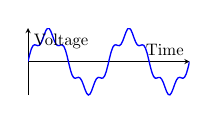
\begin{tikzpicture}[scale=0.6]
            \begin{axis}[
                xlabel={Time},
                ylabel={Voltage},
                domain=0:4*pi,
                samples=100,
                axis lines=center,
                ticks=none,
                width=5cm,
                height=3cm
            ]
            \addplot[blue, thick] {sin(deg(x)) + 0.2*sin(deg(5*x))};
            \end{axis}
        \end{tikzpicture}
        \end{center}
    \end{block}
\end{column}

\begin{column}{0.5\textwidth}
    \begin{block}{Digital Signals}
        \begin{itemize}
            \item Discrete levels (typically 2:  0 and 1)
            \item Examples: computer data, logic signals
            \item Noise immunity
            \item Requires switching circuits
        \end{itemize}
        
        \begin{center}
        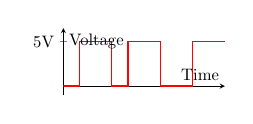
\begin{tikzpicture}[scale=0.6]
            \begin{axis}[
                xlabel={Time},
                ylabel={Voltage},
                domain=0:10,
                samples=200,
                axis lines=center,
                ytick={0, 1},
                yticklabels={0V, 5V},
                xtick=\empty,
                width=5cm,
                height=3cm,
                ymin=-0.2,
                ymax=1.3
            ]
            \addplot[red, thick, const plot] coordinates {
                (0,0) (1,0) (1,1) (3,1) (3,0) (4,0) (4,1) (6,1) (6,0) (8,0) (8,1) (10,1)
            };
            \end{axis}
        \end{tikzpicture}
        \end{center}
    \end{block}
\end{column}
\end{columns}

\vspace{0.3cm}

\textbf{This course covers both: } analog circuits (amplifiers) and digital circuits (logic gates)

\end{frame}

\begin{frame}{What is an Amplifier?}

\begin{block}{Definition}
    A circuit that increases the amplitude of a signal while (ideally) preserving its shape
\end{block}

\begin{center}
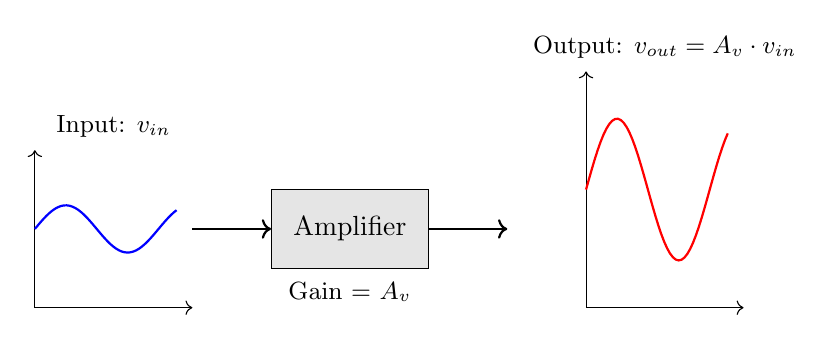
\begin{tikzpicture}
    % Input signal
    \draw[->] (0,0) -- (0,2);
    \draw[->] (0,0) -- (2,0);
    \draw[blue, thick] plot[domain=0:1. 8, samples=50] (\x, {0.3*sin(deg(4*\x)) + 1});
    \node at (1, 2. 3) {\small Input:  $v_{in}$};
    
    % Amplifier block
    \draw[fill=gray! 20] (3,0.5) rectangle (5,1.5);
    \node at (4,1) {Amplifier};
    \node at (4,0.2) {\small Gain = $A_v$};
    \draw[->, thick] (2,1) -- (3,1);
    \draw[->, thick] (5,1) -- (6,1);
    
    % Output signal
    \begin{scope}[xshift=7cm]
        \draw[->] (0,0) -- (0,3);
        \draw[->] (0,0) -- (2,0);
        \draw[red, thick] plot[domain=0:1.8, samples=50] (\x, {0.9*sin(deg(4*\x)) + 1. 5});
        \node at (1, 3.3) {\small Output: $v_{out} = A_v \cdot v_{in}$};
    \end{scope}
\end{tikzpicture}
\end{center}


\end{frame}

\begin{frame}{Why Do We Need Amplifiers?}

\begin{block}{Weak Signals Need Amplification}
    \begin{itemize}
        \item Microphone output:  ~1-10 mV
        \item Antenna signal: $\mu$V to mV range
        \item Sensor outputs: often very small
    \end{itemize}
\end{block}

\begin{block}{Examples}
    \begin{itemize}
        \item \textbf{Audio system: } Microphone → Amplifier → Speaker
        \item \textbf{Radio receiver:} Antenna → RF Amplifier → Demodulator
        \item \textbf{Communications:} Weak signal → Amplifier → Transmitter
    \end{itemize}
\end{block}

\begin{alertblock}{Key Requirement}
    Amplification must preserve signal fidelity (minimize distortion)
\end{alertblock}

\end{frame}

\begin{frame}{The Transistor:  Building Block of Electronics}

\begin{columns}
\begin{column}{0.5\textwidth}
    \begin{block}{What is a Transistor?}
        \begin{itemize}
            \item Three-terminal semiconductor device
            \item Acts as electronically controlled switch or amplifier
            \item Small signal controls large current/voltage
            \item Nonlinear device
        \end{itemize}
    \end{block}
    
    \begin{block}{Two Main Types}
        \begin{itemize}
            \item \textbf{BJT: } Current-controlled
            \item \textbf{MOSFET:} Voltage-controlled
        \end{itemize}
    \end{block}
\end{column}

\begin{column}{0.5\textwidth}
    \begin{center}
        \textbf{Simple Amplifier Concept}
        
        \begin{circuitikz}[scale=0.8]
            \draw (0,0) node[npn](npn){};
            \draw (npn.base) -- (-1.5,0) to[sV, l=$v_{in}$] (-1.5,-2);
            \draw (npn.emitter) -- (0,-2);
            \draw (-1.5,-2) -- (0,-2) node[ground]{};
            \draw (npn.collector) -- (0,1. 5) to[R, l=$R_C$] (0,3);
            \draw (0,3) to[short, -o] (0.5,3) node[right]{$V_{CC}$};
            \draw (npn.collector) to[short, -o] (1,1.5) node[right]{$v_{out}$};
            \node[above] at (0,3. 5) {\small Common-Emitter Amp};
        \end{circuitikz}
        
        \vspace{0.3cm}
        
        Small $v_{in}$ controls large $v_{out}$
    \end{center}
\end{column}
\end{columns}

\end{frame}

\begin{frame}{Linear vs.  Nonlinear Devices}

\begin{columns}
\begin{column}{0.5\textwidth}
    \begin{block}{Linear Devices (Circuits I)}
        \begin{itemize}
            \item Resistor: $v = iR$
            \item Capacitor: $i = C\frac{dv}{dt}$
            \item Inductor: $v = L\frac{di}{dt}$
        \end{itemize}
        
        \textbf{Property:} Superposition applies
        
        \begin{center}
        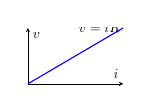
\begin{tikzpicture}[scale=0.5]
            \begin{axis}[
                xlabel={$i$},
                ylabel={$v$},
                domain=0:2,
                axis lines=center,
                ticks=none,
                width=4cm,
                height=3cm
            ]
            \addplot[blue, thick] {x};
            \node at (axis cs:  1. 5, 2) {$v = iR$};
            \end{axis}
        \end{tikzpicture}
        \end{center}
    \end{block}
\end{column}

\begin{column}{0.5\textwidth}
    \begin{block}{Nonlinear Devices (This Course)}
        \begin{itemize}
            \item Diode: $i = I_s(e^{v/V_T} - 1)$
            \item MOSFET: $i_D \propto (v_{GS} - V_{th})^2$
            \item BJT: $i_C = I_s e^{v_{BE}/V_T}$
        \end{itemize}
        
        \textbf{Property:} Superposition does NOT apply
        
        \begin{center}
        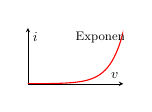
\begin{tikzpicture}[scale=0.5]
            \begin{axis}[
                xlabel={$v$},
                ylabel={$i$},
                domain=0:0.8,
                axis lines=center,
                ticks=none,
                width=4cm,
                height=3cm,
                ymin=0,
                ymax=3
            ]
            \addplot[red, thick, samples=50] {exp(10*x - 6)};
            \node at (axis cs: 0.6, 2.5) {\small Exponential};
            \end{axis}
        \end{tikzpicture}
        \end{center}
    \end{block}
\end{column}
\end{columns}

\vspace{0.3cm}

\begin{alertblock}{Challenge}
    Analysis of nonlinear circuits requires new techniques.
\end{alertblock}

\end{frame}

\begin{frame}{DC Analysis vs. AC Analysis}

\textbf{Key concept for transistor circuits:}

\begin{block}{DC (Bias) Analysis}
    \begin{itemize}
        \item Establish the operating point (Q-point)
        \item All capacitors open circuit, all inductors short circuit
        \item Determines DC voltages and currents
        \item Ensures transistor operates in desired region
        \item Uses large-signal models
    \end{itemize}
\end{block}

\begin{block}{AC (Small-Signal) Analysis}
    \begin{itemize}
        \item Analyze behavior for small variations around Q-point
        \item All DC sources set to zero (AC ground)
        \item Capacitors short circuit (at signal frequency)
        \item Uses linearized small-signal models
        \item Determines gain, impedances, frequency response
    \end{itemize}
\end{block}

\begin{alertblock}{Important}
    Both analyses are necessary for complete circuit design
\end{alertblock}

\end{frame}

\begin{frame}{SPICE Simulation}

\begin{block}{What is SPICE?}
    \begin{itemize}
        \item \textbf{S}imulation \textbf{P}rogram with \textbf{I}ntegrated \textbf{C}ircuit \textbf{E}mphasis
        \item Industry-standard circuit simulator
        \item We'll use Multisim (National Instruments)
    \end{itemize}
\end{block}

\begin{block}{Why Use SPICE?}
    \begin{itemize}
        \item Higher accuracy than pencil-and-paper calculations
        \item Explore parameter variations quickly
        \item Visualize waveforms and frequency response
        \item Test designs before building hardware
        \item Learn industry-standard tool
    \end{itemize}
\end{block}


\end{frame}

\end{document}
